\documentclass[border=3pt,tikz]{standalone}
\usepackage[utf8]{vietnam}
\usetikzlibrary{calc,angles,intersections,shapes.geometric,arrows,decorations.markings,arrows.meta,patterns.meta,patterns}
\usepackage{tikz-3dplot,pgfplots}
\pgfplotsset{compat=1.15}
\usepgfplotslibrary{polar}
\usepackage{amsmath}
\begin{document}
	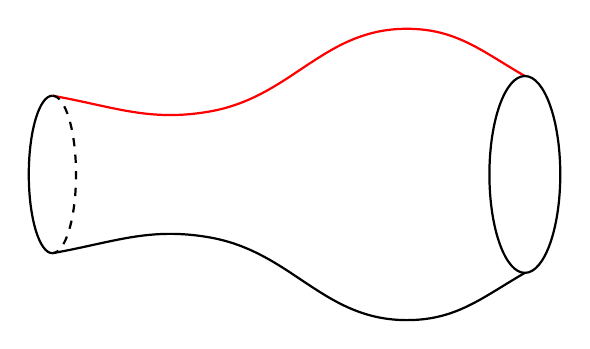
\begin{tikzpicture}[scale=1]
		\def\tpath{(1,1)to[out=350,in=190](3,0.8)to[out=10,in=180](5.5,1.85)to[out=0,in=150](7,1.25)};
		\draw[thick,red] \tpath;
		\draw[thick,yscale=-1] \tpath;
		\draw[thick] (1,1) arc(90:270:0.3 cm and 1 cm);
		\draw[thick,dashed] (1,1) arc(90:-90:0.3 cm and 1 cm);
		\draw[thick] (7,0) circle (0.45 cm and 1.25 cm);
	\end{tikzpicture}
\end{document}
